% path for images
\graphicspath{{assets/qml/}}

\section[Quantum Machine Learning]{Quantum Machine Learning}

%%
\begin{frame}{How can ML benefit from Quantum Computers ? }
	\begin{itemize}
		\item AI/ML already uses (massively) special-purpose processors: GPUs, TPUs, ASICs
		\item  Quantum computers (\alert{QPUs}) could be used as special-purpose AI
		accelerators
		\item May enable training of \alert{previously intractable} models
	\end{itemize}
\begin{figure}[H]
	\centering
	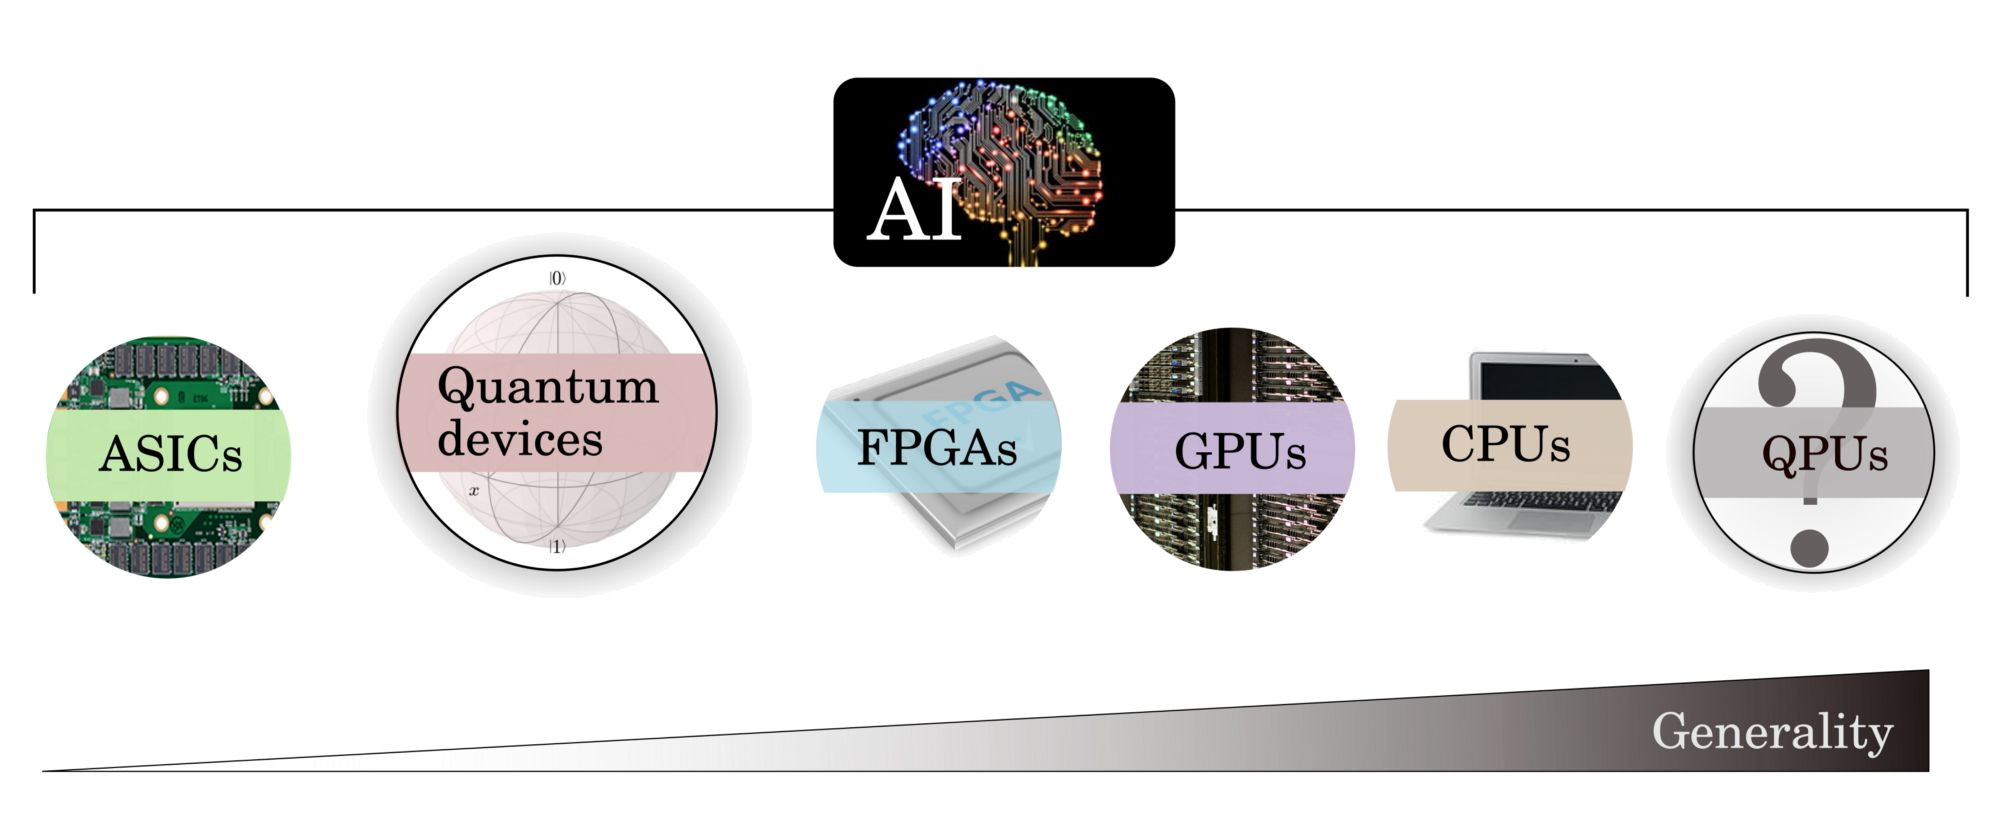
\includegraphics[width=.7\linewidth]{ qpu}
\end{figure}
\end{frame}

%%
\begin{frame}{How can ML benefit from Quantum Computers? }
	Quantum computing can also lead to \alert{new} machine learning models\\
	Examples currently being studied are:
	 \begin{itemize}
	 	\item \alert{Tensor Networks}
	 	\item Kernel methods
	 	\item Boltzmann machines
	 	\item \alert{Variational Quantum Circuits}
	 	\item Quantum Neural Networks
	 \end{itemize}
 \footnotesize
 	\begin{quantikz}
 	& \gate[wires=4][1.5cm]{U_1(\theta_1, \phi_1)}& \gate{S(r_1)} & \gate[wires=4][1.5cm]{U_2(\theta_2, \phi_2)} & \gate{D(\alpha_1)} & \gate{\Phi(\lambda_1)}  & \qw\\
 	& \qw 										& \gate{S(r_2)} &  \qw & \gate{D(\alpha_2)} & \gate{\Phi(\lambda_2)} & \qw \\ %% to leave space for the 3 dots
 	& \vdots & \vdots \ \ & \vdots & \vdots & \vdots  \\ 
 	& \qw 										& \gate{S(r_N)} & \qw  & \gate{D(\alpha_N)} & \gate{\Phi(\lambda_N)} & \qw
 \end{quantikz}
\end{frame}


%%
\begin{frame}{A lesson from Deep Learning's success}
	\begin{Large}
		Why is Deep Learning \alert{Successful} ? 
	\end{Large}

	\begin{itemize}
		\item hardware advancements(GPUs, recently TPUs)
		\item Workhorse algorithms (backprop, stochastic GD, ...)
		\item specialized, user-friendly, maintained, high-perfomance software (PyTorch, Tensorflow, Keras)
		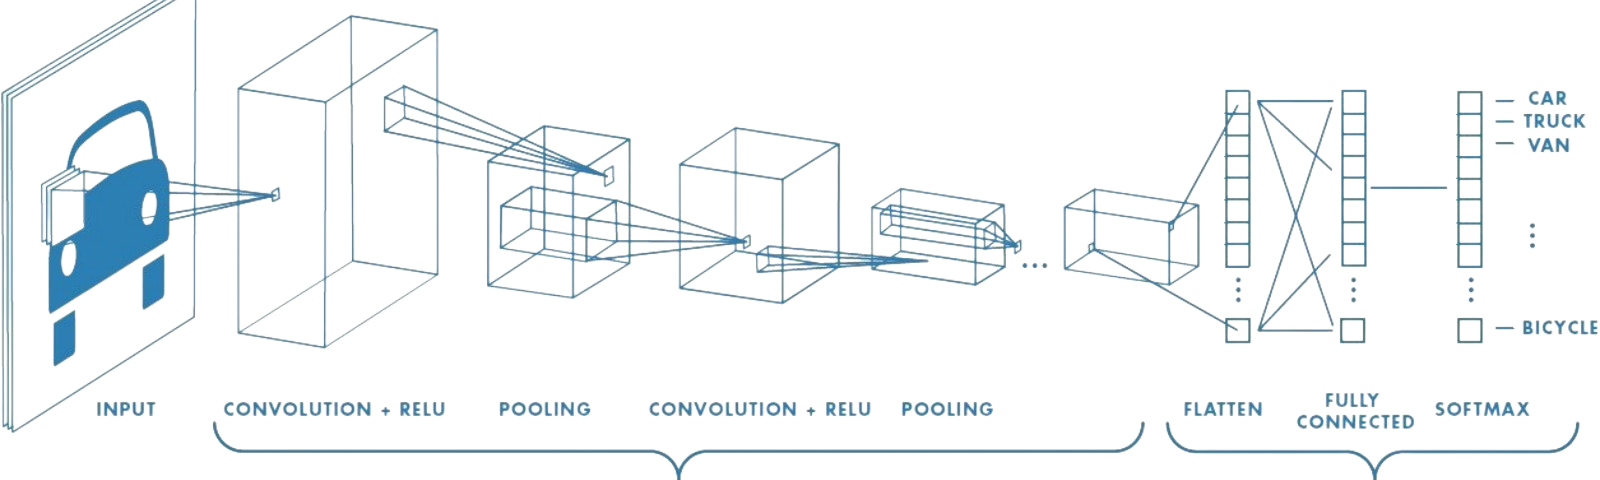
\includegraphics[width=.8\linewidth]{backprop}
	\end{itemize}	
\end{frame}

%%
\begin{frame}{What can we laverage?}
	\begin{itemize}
		\item hardware advancements(GPUs, TPUs + \alert{QPUs})
		\item 
		workhorse algorithms\\ (\alert{quantum-aware} backpropagation, stochastic GD, ...)
		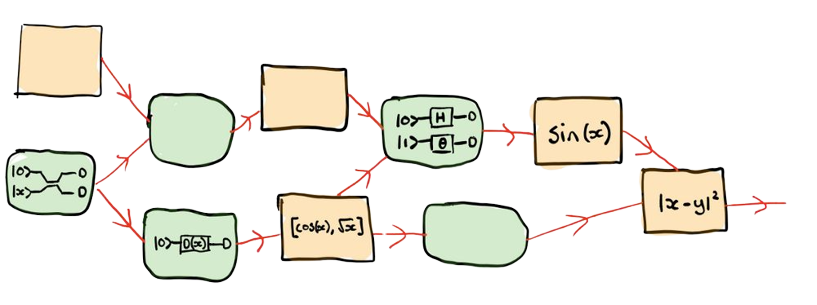
\includegraphics[width=.6\linewidth]{qbackprop}
%		\adjustbox{valign=t}{
%			\begin{minipage}[t]{0.3\linewidth}
%				workhorse algorithms (\alert{quantum-aware} backpropagation, stochastic GD, ...)
%			\end{minipage}
%		}
%		\hfill
%		\adjustbox{valign=t}{
%			\begin{minipage}[t]{0.5\linewidth}
%				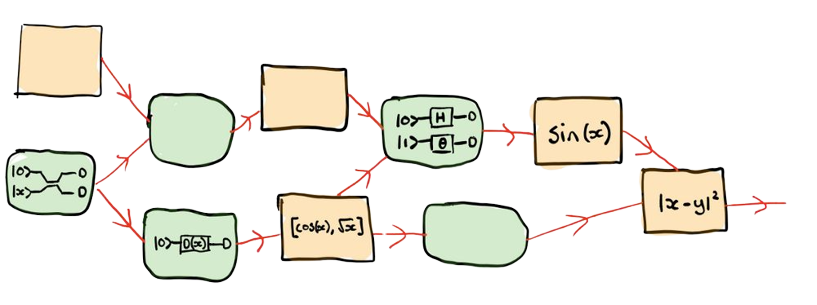
\includegraphics[width=\linewidth]{qbackprop}
%			\end{minipage}
%		}
%		
		
		
		
		\item specialized, user-friendly, high-performance software (Pennylane, Qiskit, Tensorflow Quantum, ...)
		
		\item 
		\alert{hybrid} computation\\
		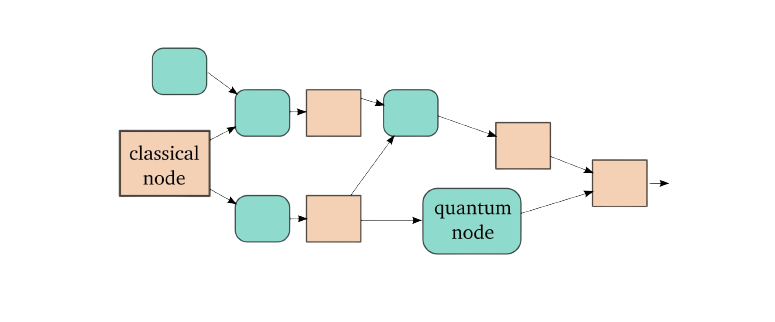
\includegraphics[width=.7\linewidth]{hybrid}
		
	\end{itemize}
\end{frame}